% Chapter Template

\chapter{Introduction} % Main chapter title

\label{Chapter1} % Change X to a consecutive number; for referencing this chapter elsewhere, use \ref{ChapterX}

This thesis is the final documentation for a project in the Master of Science degree of High Integrity Systems supervised by Prof. Dr. Peter Thoma and Prof. Dr. Egbert Falkenberg. In this thesis, the author will explain the basics of electromagnetic simulation and demonstrate a simple application that will produce both electric and magnetic field data, which can then be visualized through the help of third party applications such as Paraview\textsuperscript{\cite{paraview}}. 

This thesis is heavily focused on theoretical aspect of such an application, and as such the code will be simplistic and not use any advanced external libraries not included by default in standard C++. The application will not have a User Interface (UI), therefore the only way to customize the initial values of the code variables would be through an Integrated Development Environment (IDE) that can handle C++, such as Eclipse \textsuperscript{\cite{eclipse}}. The benefit of not relying on any external open source libraries is the ability for this code to be used by any machine regardless of operating system and easy integration into applications that need such simulations.

Alongside this document, the project also included the code files found in the GitHub repository\textsuperscript{\cite{robo}}. As the base \LaTeX \space template of this thesis was found online\textsuperscript{\cite{template}}, these files are also included, with the license allowing viewing and modification so long as it is for a non-commercial use. After the official deadline of January 5th 2021, this project will be considered complete and no further changes will be made.

\section{Motivation}

As humanity strives to better understand the world and universe around it, the physical limitations become more and more apparent. While people have made considerable progress in their struggles to move forward, such as being able to record the movement of a light particle on camera despite it being the fastest moving object known of so far\textsuperscript{\cite{velten2013femto}}, or being able to capture an image of a black hole\textsuperscript{\cite{landau_2019}}, such achievements would not have been possible if scientists did not have realistic expectations of how they should approach these challenges, or the expected results. 

In order to achieve what they have, scientists needed to first understand the phenomena they were studying: the light having the particular properties of both particle and wave and the ability of black holes to distort space around them. All of this would not have been possible without simulations. 

This thesis is going to describe the implementation of a C++ algorithm that uses the FDTD method to simulate how an electromagnetic field behaves in vacuum. The goal of the app is to be able to generate data that can then be used by a third party visualization program. This project features three standalone implementations, for one-dimensional, two-dimensional, and three-dimensional cases.

The basis for all of these calculations are the well known Maxwell Equations, which govern all electromagnetic phenomena. They will be used alongside the FDTD method to create update equations that will run in a loop for a certain amount of time. The initial values, domain size, domain environment, and simulation time can all be changed in code. To begin off the simulation, a starting impulse will be eeded. For this project, the Gaussian pulse equation will be adapted used to add an excitation to the simulation that would otherwise be static. 

At the end, one can find the conclusion where uses for this application as well as further improvements are discussed. Anyone that would like to use this project as a basis for their own work should take a look at the \ref{AppendixA} should they have any issues.

%----------------------------------------------------------------------------------------
%	SECTION 1
%----------------------------------------------------------------------------------------

\section{Electromagnetic Simulations}
With the fast development of technology came new opportunities for gaining a better understanding of vast natural phenomena. This thesis will be focusing on one of them, that being Electromagnetic Wave Propagation. 

As one can imagine, analyzing electromagnetic fields through plain observation is near impossible, with only a few exceptions\textsuperscript{\cite{cao2005first}}. Even if one supposed that it was possible to easily achieve an acceptable amount of information from observing experiments, the cost and quality of the resulting data would mostly be of scientific use, with little to no practical use whatsoever. Considering that electromagnetic waves are widely used in almost every industry, either as part of the building process or as a finished product, having data that cannot be used practically does not help. 

That is why, thanks to the progress made in the computational capabilities of computers so far and the use of the theories and formulas gathered from past scientific endeavors, one can create data that is a close approximate of reality. Both shall be discussed in this chapter, but one cannot proceed without first going into the equations that govern large-scale electromagnetic phenomena in static mediums\textsuperscript{\cite{stratton2007electromagnetic}}: Maxwell Equations.

%-----------------------------------
%	SUBSECTION 1
%-----------------------------------
\subsection{Maxwell Equations}

As mentioned above, Maxwell Equations are believed to dictate the behavior of all kinds of electromagnetic fields at a macroscopic level. These equations are the following:

\begin{equation}
	\label{eqn:electricinduction}
	\vec{\nabla} \times \vec{E}(\vec{r},t) = - \frac{\partial \vec{B}(\vec{r},t)}{\partial t}
\end{equation}
\begin{equation}
	\label{eqn:amperesLaw}
	\vec{\nabla} \times \vec{H}(\vec{r},t) = \vec{J}(\vec{r},t) + \frac{\partial \vec{D}(\vec{r},t)}{\partial t}
\end{equation}
\begin{equation}
	\label{eqn:magneticDivergence}
	\vec{\nabla} \cdot \vec{B}(\vec{r},t) = 0
\end{equation}
\begin{equation}
	\label{eqn:gausslaw}
	\vec{\nabla} \cdot \vec{D}(\vec{r},t) = \rho (\vec{r})
\end{equation}

To give a brief explanation over the meaning of each equation:

Equation \ref{eqn:electricinduction} explains the effects of the electric field $\vec{E}$ on the rate of change of the magnetic induction $\vec{B}$. This can also be referred to as the equation of electromagnetic induction, where the right hand side is the EMF or voltage and the left hand side is the magnetic flux. To those who study this particular area of physics, this equation will seem familiar, because it was derived from Faraday's law of induction.

\begin{figure}
	\centering
	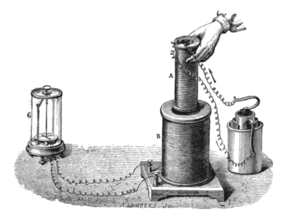
\includegraphics{Figures/faradayexp}
	\decoRule
	\caption[Faraday's Experiment]{Faraday's Experiment,\textsuperscript{\cite{poyser1918magnetism}}} which resulted in the law that was later used by Maxwell in making his equation.
	\label{fig:faradayexp}
\end{figure}

Equation \ref{eqn:amperesLaw} is also known as Ampère–Maxwell law, because although it originated from Ampère, the current form was derived by Maxwell to include the magnetic current density $\vec{J}$. The equation explains the effects of the magnetic field on the electric current.

Equation \ref{eqn:magneticDivergence}, otherwise known as Gauss's law for magnetism, talks about the divergence of the magnetic field. According to this law the divergence is always 0. What this means is that in a magnetic field there is no such thing as a source (positive divergence) or a sink (negative divergence), rather a magnetic field can be more closely compared to a closed loop that flows in one direction. That is why every magnet that is known so far, at least under normal conditions, of has two poles. To translate this into something more easily understandable, it basically means that, if one was to pick any subset of the area of a magnetic field, no matter what area was picked, it would have the same number of vector fields going inside and out. A simple representation of this rule can be seen in \ref{fig:magneticdivergence}, where it can be noted that the number of vectors heading towards the north pole are equal to the vectors going outside of it. Interestingly enough, if the bar magnet were to be cut in half, then the result would be two smaller bar magnets with 2 poles each and the exact same vector field.

\begin{figure}
	\centering
	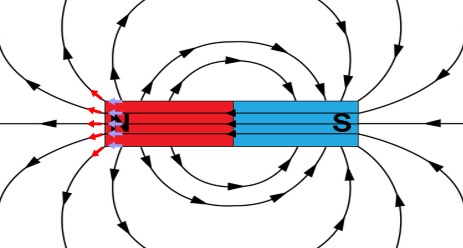
\includegraphics[scale=0.9]{Figures/magneticdivergence}
	\decoRule
	\caption[Magnetic Divergence]{A crude representation of magnetic divergence through the use of a bar magnet.}
	\label{fig:magneticdivergence}
\end{figure}

Equation \ref{eqn:gausslaw}, is the main Gauss law for electric currents. It looks rather similar to his law of magnetism on the left hand side; the previous magnetic divergence is now replaced with the electric divergence. The bigger difference is the $\rho$ on the right hand side, which is the density of charge of the electric field. In basic terms, it means that the divergence of the electric field is equal to the charge density for that point.

For the above equations, the following material relations will be useful later on:
\begin{equation}
	 \vec{D}(\vec{r},t) = \epsilon(\vec{r}) \cdot \vec{E}(\vec{r},t)
\end{equation}
\begin{equation}
	\vec{B}(\vec{r},t) = \mu(\vec{r}) \cdot \vec{H}(\vec{r},t)
\end{equation}

The equations above are shown in their derivative form, but they can also be shown as their integral equivalent. There is no difference in implementation, regardless of which form is used.

%-----------------------------------
%	SUBSECTION 2
%-----------------------------------

\subsection{Solving the Wave Equation}
Using the formulas above, one can derive the electromagnetic wave equation, which is needed to proceed with the implementation further. Firstly for convenience, an assumption will be made that the environment is the vacuum of space. Secondly, it can also be assumed that there is no initial charge in this space or loss of energy. This means that $\epsilon(\vec{r})=\epsilon_{0}$ and $\mu(\vec{r})=\mu_{0}$. This allows for the simplification of the above equations and gives the numerical solution for the wave equation:

\begin{equation}
	\label{eqn:waveEquation}
	\Delta\vec{E}(\vec{r},t) - \frac{1}{c^2} \frac{\partial^2 \vec{E}(\vec{r},t)}{\partial t^2} = \mu_{0} \frac{\partial \vec{J}(\vec{r},t)}{\partial t},
\end{equation}

where: $$c = \frac{1}{\sqrt{\mu_{0}\epsilon_{0}}}$$

This equation is useful because it will be used to derive the formulas that are going to be needed for the simulations. Going forwards, this will be used as a basis to adapt the solution to every environment, regardless of dimensionality. From this point, there are many ways to proceed. Some of the most notable are the Finite Element Method (FEM), the Finite Integration Technique (FIT), and the Finite Difference Time Domain Method (FDTD). All of them are also known as Approximation Methods.

FEM is a well known numerical method used to obtain an approximation for a given boundary value problem. The basic principle is to divide a system into smaller subsets, called finite elements (hence the name), which are much simpler to solve. This is done by discretizing the given space for each of its dimensions, and then constructing a mesh of the object. As a result, from the initial boundary value problem one can get a system of equations that are further used to approximate each singular simplified function over the given domain. These equations are then compiled together into a system of equations that is then used to model the initial problem. The solution is then approximated by solving this system and minimizing the error function.\textsuperscript{\cite{logan2011first}}

The finite integration technique (FIT) is a bit more straightforward. It can help numerically solve electromagnetic field problems by disctretizing in both the time and frequency domain. The first to introduce this technique was Thomas Weiland in 1977.\textsuperscript{\cite{weiland1977discretization}} It has later seen continuous improvements and can now cover all electromagnetic problems and applications. This approach works by using the Maxwell equations above and applying their integral form to a set of staggered grids (e.g. Cartesian grid). This allows for a memory efficient implementation as well as giving the ability to handle different boundary conditions and variable material properties.

Finally there exists a well known computational electromagnetic technique used for approximation, the Finite Difference Time Domain Method. It is arguably the easiest method out of the three to understand and implement, which is surprising when considering the capabilities it has in solving wave equations. 

This simplicity is also the reason it was chosen for this thesis, as it is the only technique that one person can realistically implement by themselves in a reasonable time frame.\textsuperscript{\cite{davidson2010computational}} It is also worth noting that FIT can be used for deriving the update equations that will be used in the FDTD algorithm. As the name implies this is a time-domain method, meaning that a wide range of frequencies can be covered with a single simulation run. The only caveat is that the time step needs to be small enough to not cause any instabilities in the system.

%----------------------------------------------------------------------------------------
%	SECTION 2
%----------------------------------------------------------------------------------------

\section{Finite Difference Time Domain Method}

FDTD was first proposed by Kane Yee in a 1966 paper and was initially called the Yee Algorithm, taken from the author's name. It was modified later from further research, resulting in the modern version that is widely used to this day. This method can be basically summarized in the following steps:

\begin{enumerate}
	\item Replace the derivatives from the Maxwell Equations with finite differences
	\item Discretize the space and time of the domain, while staggering the electric fields from the magnetic ones (e.g. by half a time step, and spatially by using a different axis)
	\item Get the update equations
	\item Use the update equations to get the future step for magnetic and electric fields
	\item Repeat the step above throughout the set duration
\end{enumerate}

The most important steps are 2 and 3, as the rest are relatively easy to do and it is highly unlikely for any mistakes to occur, especially once this is implemented in code. The next section will go quickly through the first step, which will the basis that will be used moving forward. Steps 2-5 are implementation specific and vary depending on the domain. As such, they will be explained for each scenario in their respective chapters.

\section{FDTD Implementation}

Before beginning with the discretization, it was mentioned previously that Maxwell's Equations can be shown in both their differential form and their integral form. Using this form has the benefit that the equations are easier to work with and follow. Using integrals instead of derivatives, however, does mean that, at least for the derivation, FIT is being used instead of FDTD. Despite that, the final equations will be the same. Here is the integral form of Maxwell's Equations:


\begin{equation}
	\label{eqn:electricinductionintegral}
	\oint E \cdot ds = - \frac{d}{dt} \int B \cdot dA
\end{equation}
\begin{equation}
	\label{eqn:amperesLawintegral}
	\oint H \cdot ds = \int \frac{dD}{dt} \cdot dA
\end{equation}
\begin{equation}
	\label{eqn:magneticDivergenceintegral}
	\int D \cdot dA = \int \rho dV
\end{equation}
\begin{equation}
	\label{eqn:gausslawintegral}
	\int B \cdot dA = 0
\end{equation}

The material relations will look as follows:

\begin{equation}
	\label{eqn:dIntegral}
	D = \epsilon \cdot E
\end{equation}
\begin{equation}
	\label{eqn:bIntegral}
	B = \mu \cdot H
\end{equation}

By plugging \ref{eqn:bIntegral} and \ref{eqn:dIntegral} into equations \ref{eqn:electricinductionintegral} and \ref{eqn:amperesLawintegral} respectively:

\begin{equation}
	\label{eqn:electricUpdateIntegral}
	\oint E \cdot ds = - \frac{d}{dt} \int \mu \cdot H \cdot dA
\end{equation}
\begin{equation}
	\label{eqn:magneticUpdateIntegral}
	\oint H \cdot ds = \frac{d}{dt} \iint \epsilon \cdot E \cdot dA
\end{equation}

Equations \ref{eqn:electricUpdateIntegral} and \ref{eqn:magneticUpdateIntegral} are going to be used later on during the implementation to derive the specific update equations. With all that, the general theoretical part is finished. For this project, the above functions will need to be implemented into a program that can generate approximate data on electromagnetic waves, which will be discussed in the next section.

\subsection{Application Requirements}

The result of this project is not only this documentation, but also a relatively simple program that can be used either as is, or implemented into a bigger project with minor adjustments. As such, the resulting application must adhere to the following requirements:

\begin{itemize}
	\item Allow for the generation of electromagnetic data in a set environment (e.g. vacuum)
	\item Have a smooth impulse to start off the simulation
	\item Use only the standard C++, no external dependencies
	\item Support one dimensional, two dimensional, and three dimensional domains.
	\item Be simple and compact, so that it can be adapted to a bigger application if necessary
\end{itemize}

The first requirement is understandably the most basic functionality, the goal of the whole project. This data will be generated from scratch, using the environment variables of permittivity $\epsilon$ and permeability $\mu$. These values can be changed depending on the environment, which can be vacuum, copper, etc. The examples here will use the values for free space $\epsilon_{0}$ and $\mu_{0}$. Also, these values are going to be constant throughout the simulation, meaning it will feature one material through out the whole domain. 

Without a starting impulse, there would be nothing to simulate, as the data would simply keep its initial value of zero. If one was to add an immediate pulse of an arbitrary value to a single point, it would prove sufficient. However, this would result in a sudden explosion of a single electromagnetic pulse that would simply travel along the domain as a single point, thus providing a near useless visualization once the data is put into an appropriate program. 

Instead, the Gaussian pulse excitation can be used in the middle of the domain, and have it propagate throughout it. This is ideal because the simulation is using reflective boundaries, meaning the pulse will bounce back and forth between each boundary without any loss. If one was to use absorbing boundary conditions, such an excitation would eventually lead to the waves disappearing completely. For such cases, a steady sinusoidal excitation that keeps going would prove more interesting.

A Gaussian pulse will be used for this example. The generic formula is given below:

\begin{equation}
	\label{eqn:gaussianPulse}
	f(t) = \alpha e^{-\beta(t - T_\varepsilon/2)^2}
\end{equation}
where
\begin{equation}
	\label{eqn:gaussianBeta}
	\beta = - (\frac{2}{T_\varepsilon})^2 \ln\varepsilon
\end{equation}

A good value for sufficient smoothness would be $\varepsilon = 0.001$, but this is heavily dependent on the implementation.

For the third requirement, the reason why this project would want to avoid the use of header files that are not included by default in C++ is that such files could make the program dependent on things such as the operating system that the machine is running, PATH variables, etc. In short, it would complicate the setup to run such a program too much, possibly voiding the last requirement. On top of that, in insisting on using only the very basics that C++ has to offer, the resulting code will be easier to relate to the formulas that are shown in this thesis, since all the code will be visible at all times. With that said, various improvements could be made if the use of external libraries is allowed. That will be discussed in more details in the Conclusion.

Fourth, the application should support anything from one to three dimensions. While only a 3D simulation would be realistically desired, for a thesis the 1D and 2D scenarios are also interesting to study. Not only that, but the 1D application leads smoothly to the development of the 2D application, which in turn leads to the smooth development of the 3D application. This progression resulted in having a standalone program for each scenario, rather than one for all of them. Rather than unify these applications, they were intentionally left as separate programs in the end, because it helps in complying with the last requirement.

Lastly, after going through each of the previous requirements, this one is rather self-explanatory. To begin with, simple and compact code that works well standalone is one of the most important programming practices that developers should follow. While this program's goal is to simply be used as a demonstration of such an implementation, it should also be easily modifiable and adaptable, so that it can provide a good basis that can be used by larger applications that include far more features.

With that said, certain limitations that plague all computers, simply due to their nature, will have to be explained. Since these limitations cannot be bypassed as of yet, one can never achieve an exact, perfectly realistic simulation. Thus, it is good to keep them in mind while developing such applications.

\subsection{Computational Limitations and Inaccuracies Explained}

Programmers can use programming languages to instruct computers to perform certain commands in certain orders, thus creating applications. However, these instructions are not what the computers use to dictate what should happen. These programming languages are decoded by the interpreter of choice, and then passed down in the form of a lower level language. This process occurs more than once too, until one gets to the smallest unit a computer can have: a bit.

A bit is simple; it can have either a value of zero or one. Instructions are basically translated into many such bits, thus making what is basically computer language. Each instruction could be translated into millions of bits, but that by itself would not cause issues normally. The issue is that, no matter how powerful the computer is or how much memory it has, these bits are finite. As such, they present limitations when dealing with infinite concepts.

One such concept is infinite numbers. This would be best explained with an example: summing fractions into a whole. If a person was to be asked to add $\frac{1}{9}$ nine times, they would do the following:
$$\frac{1}{9} + \frac{1}{9} + \frac{1}{9} + \frac{1}{9} + \frac{1}{9} + \frac{1}{9} + \frac{1}{9} + \frac{1}{9} + \frac{1}{9} = 1 \;,$$ which a person knows is correct. However, when one runs the following code snippet:

\begin{minted}[breaklines,frame=single]{c++}
	double a = 1.0/9.0;
	if (a + a + a + a + a + a + a + a + a == 1.0) {
		cout << "Equal to 1";
	} else {
		cout << "Not equal";
	}
\end{minted}

one would get the following result (Fig. \ref{fig:finiteprecision}): 
\begin{figure}[h!]
	\centering
	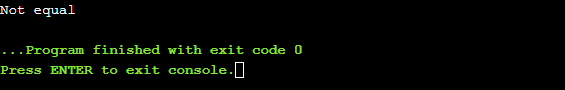
\includegraphics{Figures/finiteprecision}
	\decoRule
	\caption[Code Result]{According to the code, the total sum is not equal to 1.0, even though it should be.}
	\label{fig:finiteprecision}
\end{figure}

What is happening is that a computer is being asked to store the infinite number $1/9 = 0.\overline{1}$ using a finite amounts of bit. Depending on the data type that is used, it can have anywhere from 8 bits of precision, to $2^8$ bits. However, that is still a finite amount, and no matter what one does, the resulting value will be truncated to $0.1111...1$, resulting in a sum of $0.9999...9 \neq 1.0$ . That is why any simulation, regardless of the computer or the method used, will always be an approximation of reality. When performing thousands of calculations, this margin of error increases further. Despite that, these approximations are enough to give a good idea of what to expect. Even more so when considering that there is an error with even bigger margins that must be discussed.

\subsection{Discretization Error\textsuperscript{\cite{roy2010review}}}

In computer simulations, by far the most noteworthy type of error is the Discretization Error. This error occurs whenever a discretization technique is applied. In more conventional words, it occurs whenever a continuous function or phenomenon is calculated as a finite number of evaluations using a  computer (Figure \ref{fig:discretizationError}).

\begin{figure}[h!]
	\centering
	\includegraphics{Figures/discretizationError}
	\decoRule
	\caption[Discretization Error]{The difference between various estimations and the exact result\textsuperscript{\cite{dow_1998}}}
	\label{fig:discretizationError}
\end{figure}

This type of error is inevitable whenever approximation techniques are used. In FDTD, it is the difference between the exact partial differential equation and the discretized algebraic equation used by the implementation. It can theoretically be calculated by taking the value of the exact solution and comparing it with the value received by the numerical approximation. In practice, however, doing so can prove difficult depending on the scenario. Such an error can also be observed by changing the domain mesh size. The smaller the mesh, the larger the error would be. 

Therefore a balance should be struck between having a small enough mesh and having a short enough computational time. Another compromise would be a variable mesh size if the areas that need high precision are known beforehand. Keeping a coarse mesh in general and only refining it where needed could aid in reducing the error margin considerably.  Alternatively, one could look at refinement methods. However, they too bear a computational cost, and will therefore not be used here.
